\section{Thursday, May 16}

\todaybox{We will give a general formula for the $n^{\text{th}}$ roots of a complex number.

We will start discussing functions, and multi-valued functions. We will discuss the exponential function $e^z$ and the trigonometric functions $\sin(z)$ and $\cos(z)$.}


\begin{thmbo}{Existence of $n^{\text{th}}$ Roots}{rootsExist}\index{Roots} 
Let $w = re^{i\theta} \in \C$. If $w = 0$, then $z^n = w$ has a unique solution, $z = 0$.

If $w\ne 0$, then the solutions to $z^n = w$ are:
$$z_j = \sqrt[n]{r}e^{\frac{i(\theta + 2j\pi)}{n}}$$

\noin where $j \in \Z$. Furthermore, it is enough to assume $j\in \{0,1,2,\dots,n-1\}$.
\end{thmbo}

\begin{proof} When $w = 0$, the claim is clear.

For $w\ne 0$, what do we need to show? We need:

\begin{itemize}
\item The $z_j$ are solutions to $z^n = w$. I.e., $z_j^n = w$.
\item The $z_j$ are the only solutions to $z^n = w$. I.e., if $z^n = w$, then $z = z_j$ for some $j$.
\end{itemize}

In other words, we need to prove that $z^n = w$ if and only if $z = z_j$ for some $j$. Let $z = se^{i\Psi}$ be in polar form. Then $z^n = w \iff  s^ne^{in\Psi} = re^{i\theta}$. This occurs if and only if $s^n = r$ and $n\Psi = \theta + 2k\pi$ for some $k\in \Z$, by considering the moduli and arguments of each side.

As such, $z^n = w$ if and only if $s = \sqrt[n]{r}$ and $\Psi = \frac{\theta + 2k\pi}{n}$ for some $k\in \Z$. I.e., $z^n = w$ if and only if $z = z_k$ for some $k\in \Z$.


Lastly, we need to justify why we only need to consider $j\in \{0,1,\dots,n-1\}$. Let $k\in \Z$. Then by the division algorithm, we can write $k = qn + j$ for some $0 \le j \le n-1$. We find that:

$$z_k = \sqrt[n]{r}e^{i\frac{\theta + 2k\pi}{n}} = \sqrt[n]{r}e^{i\frac{\theta + 2(qn + j)\pi}{n}} = \sqrt[n]{r}e^{i\frac{\theta+2j\pi}{n} + 2q\pi i} = \sqrt[n]{r}e^{i\frac{\theta + 2j\pi}{n}} = z_j$$

As such, each $z_k$ is actually equal to some $z_j$, where $0\le j \le n-1$.


Also, note that each of the $z_j$ for $j\in \{0,1,\dots,n-1\}$ are distinct. Since $\frac{\theta + 2j\pi}{n} \in \left[\frac{\theta}{n},\frac{\theta}{n} + 2\pi\right)$, we see that these angles all point in different directions.







%
%To begin, for $w\ne 0$, we should show that $z_j$ is a solution to $z^n = w$. I.e., we should show that $z_j^n = w$. However, we quickly see that 
%
%\begin{align*}z_j^n &= \left(\sqrt[n]{r}e^{\frac{i(\theta + 2j\pi)}{n}}\right)^n\\
%&= \sqrt[n]{r}^n \left(e^{\frac{i(\theta + 2j\pi)}{n}}\right)^n\\
%&= re^{\frac{in(\theta + 2j\pi)}{n}}\\
%&= re^{i(\theta + 2j\pi)} \\
%&= re^{i\theta}\\
%&= w\end{align*}
%
%Therefore, these $n$ distinct complex numbers are solutions to $z^n = w$. I leave it as an exercise for you to show they are distinct.
%
%
%Are these the only solutions?
%
%I have two arguments for you to show this.
%
%
%\paragraph{Polar form argument.} Suppose $z = |z|e^{i\Psi}$ satisfies that $z^n = w$. Then $w = z^n = |z|^ne^{in\Psi}$. However, we also know that $w = re^{i\theta}$.
%
%Now, since these complex numbers are equal, it must be that $r = |w| = |z^n| = |z|^n$, and so $|z| = \sqrt[n]{r}$.
%
%Furthermore, for these two complex numbers to be equal, they must be pointing in the same direction. I.e., $\theta$ and $n\Psi$ are arguments for the same complex number. This tells us that $n\Psi = \theta + 2k\pi$ for some $k\in \Z$. As such, $\Psi = \frac{\theta + 2k\pi}{n}$ for some $k\in \Z$.
%
%To see that we need only consider $j \in \{0,1,2,\dots, n-1\}$, note that for any $k\in \Z$, there exists $q,r\in \Z$ with $k = qn + r$ and $r\in \{0,1,2,\dots,n-1\}$, by division. Then $e^{i\frac{\theta + 2k\pi}{n}} = e^{i\left(\frac{\theta}{n} + \frac{2(qn+r)\pi}{n}\right)} = e^{i\left(\frac{\theta + 2r\pi}{n}\right) + i2q\pi} = e^{i\left(\frac{\theta + 2r\pi}{n}\right)}$. Therefore, each $k\in \Z$ yields the same root as one of the $z_j$.
%
%\paragraph{Algebra argument.} There is a much simpler argument, if we allow ourselves to stray a bit beyond the material of the course. Consider the polynomial $p(z) = z^n - w$. Over a field, a polynomial of degree $n$ has a most $n$ roots. However, we have shown that $p(z_j) = z_j^n -w = 0$ for $j = 0,1,2,\dots, n-1$. As such, we have given $n$ different roots for a degree $n$ polynomial. That must be all of the roots, and hence all the solutions to $z^n = w$.


\end{proof}

\begin{ex}{}{} Let $w = i$. Find all solutions to $z^2 = w$ and $z^4 = w$.


To begin, we need to write $w$ in polar form. In this case, it is simple: $w = e^{i\frac{\pi}{2}}$. The theorem gives us a formula for these roots.

To solve $z^2 = w$, we consider $z_0 = \sqrt{1}e^{i\frac{\pi/2}{2}} = e^{i\frac{\pi}{4}} = \frac{1}{\sqrt{2}} + \frac{i}{\sqrt{2}}$.

The other root is much easier to find. Notice that the other root is $z_1 = e^{i\frac{\pi/2 + 2\pi}{2}} = e^{i\frac{\pi/2}{2}}e^{\frac{2\pi}{2}} = -z_0$.

In solving $z^4 = w$, we can take a similar approach. Indeed, we have that $z_j = z_0e^{i\frac{2j\pi}{4}}$. This gives us a list:

\begin{itemize}
\item $z_0 = e^{i\frac{\pi}{8}}$
\item $z_1 = z_0e^{i\frac{2\pi}{4}} = iz_0$
\item $z_2 = z_0e^{i\frac{2*2\pi}{4}}= -z_0$
\item $z_3 = -iz_0$
\end{itemize}

As an interesting aside, it turns out that $e^{i\frac{\pi}{8}} = \frac{\sqrt{2 + \sqrt{2}}}{2} + i\frac{\sqrt{2 - \sqrt{2}}}{2}$. One possible way to show this would be to try to solve the equation $z^2 = \frac{1}{\sqrt{2}} + \frac{i}{\sqrt{2}}$ by setting $z = a + bi$.
\end{ex}

Notice, in our example, we factored $z_j$ as $\sqrt[n]{r}e^{i\frac{\theta}{n}}e^{i\frac{2j\pi}{n}}$. These numbers $e^{i\frac{2j\pi}{n}}$ are the $n^{\text{th}}$ roots of unity.

\begin{defbo}{Roots of Unity}{rootsUnity}\index{Roots!of unity}
The $n^{\text{th}}$ roots of unity are the solutions to $z^n = 1$. They are precisely the complex numbers $\omega_j = e^{i\frac{2j\pi}{n}}$.
\end{defbo}

\subsection{Geometry of roots}\index{Roots!geometry}

There are two nice geometric facts about the $n^{\text{th}}$ roots of $w$ that we can glean from this result.

\begin{itemize}
\item Notice that $|z_j| = \sqrt[n]{r}$ for each $j$. This means that each of the $n^{\text{th}}$ roots of $w$ all lay on the circle of radius $\sqrt[n]{r}$ centered at $0$.

This circle has the equation $|z| = \sqrt[n]{r}$. More generally, a circle of radius $r$ centered at $z_0$ has the equation $|z-z_0| = r$. \index{Circle}

\item Notice that the angle between $z_j$ and $z_{j+1}$ is exactly $\frac{2\pi}{n}$.

So, for example, the $6$th roots of $w$ form a picture like:

\begin{center}
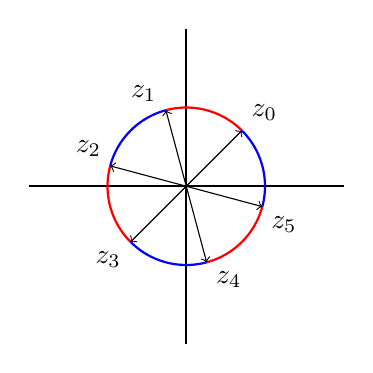
\begin{tikzpicture}
%\draw [help lines,black!20!white] (-1,-1) grid (4,4);

\draw[thick] (0,-2) -- (0,2);
\draw[thick] (-2,0) -- (2,0);


\draw [red,thick,domain= 45:105] plot ({cos(\x)}, {sin(\x)});
\draw [blue,thick,domain= 105:165] plot ({cos(\x)}, {sin(\x)});
\draw [red,thick,domain= 165:225] plot ({cos(\x)}, {sin(\x)});
\draw [blue,thick,domain= 225:285] plot ({cos(\x)}, {sin(\x)});
\draw [red,thick,domain= 285:345] plot ({cos(\x)}, {sin(\x)});
\draw [blue,thick,domain= 345:405] plot ({cos(\x)}, {sin(\x)});

\foreach \x in {0,1,...,5}
	\draw[->] (0,0) -- ({cos(45 + 60*\x)},{sin(45 + 60*\x)}) node [inner sep = -2pt, label = {[label distance = -1pt]{45 + 60*\x}:$z_\x$}]{};



\end{tikzpicture}
\end{center}

Where the arc between $z_j$ and $z_{j+1}$ has angle $\frac{\pi}{3}$. Notice that this is a regular hexagon!

\begin{center}
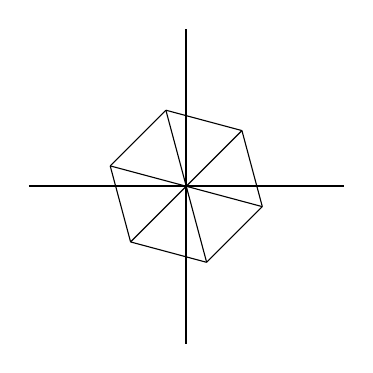
\begin{tikzpicture}
%\draw [help lines,black!20!white] (-1,-1) grid (4,4);

\draw[thick] (0,-2) -- (0,2);
\draw[thick] (-2,0) -- (2,0);

\foreach \x in {0,1,...,5}{
	\draw (0,0) -- ({cos(45 + 60*\x)},{sin(45 + 60*\x)});
	\draw ({cos(45 + 60*\x)},{sin(45 + 60*\x)}) -- ({cos(105 + 60*\x)},{sin(105 + 60*\x)});}



\end{tikzpicture}
\end{center}

And this is true in general. If $w\ne 0$ and $n\ge 3$, then the roots of $z^n = w$ form a regular $n$-gon.

\end{itemize}


I made a small note in the preceeding discussion which I would like to expand upon. Namely, how to describe complex circles.

\begin{thmbo}{}{rootsCircle}
The set of points $\{z\in\C| |z - z_0| = r\}$ is a circle of radius $r$ centered at $z_0$.
\end{thmbo}

\begin{proof} The circle of radius $r$ centered at $(x_0,y_0)$ in $\R^2$ is described by the equation $(x-x_0)^2 + (y-y_0)^2 = r^2$. We wish to show that $|z-z_0| = r$ is equivalent to this expression.

Suppose $z = x + iy$ and $z_0 = x_0 + iy_0$. Then:

$$r = |z-z_0| = |(x-x_0) + i(y-y_0)| = \sqrt{(x-x_0)^2 + (y-y_0)^2}$$

Squaring both sides gives the desired result.
\end{proof}


\begin{note} We are skipping section 1.3 in Fisher for now. It discusses the topology of $\C$. This will eventually be important, once we start talking about differentiation. For now, we can leave it.\end{note}



\subsection{Functions}

We want to be able to talk about complex calculus, so we need some notion of a function. 

\begin{defbo}{Function}{function}\index{Function}\index{Function!domain}\index{Function!range}
Let $U,W$ be subsets of $\C$. A function $f:U\rightarrow W$ is a rule that assigns to each element $z\in U$ exactly one element $f(z) \in W$. $U$ is called the domain of $f$, and $W$ is called the codomain of $f$.

The range of $f$ is the set $\{f(z)|z\in U\}$.
\end{defbo}

So, in essence, functions of a complex variable are defined exactly the same way any other function is. The difference here is that the domain and codomain both lie in planes, so we won't be able to draw to represent our functions.

\begin{ex}{}{} Find the domain and range of the function $f(x + iy) = \frac{ix + y}{x - iy}$.

When finding the domain of a function given by a formula, take the largest set on which that formula makes sense. So, in this example, the formula gives an output whenever $x - iy\ne 0$. I.e., when $z\ne 0$. So, the domain of this function is $\C\setminus\{0\}$.

For the range, $w$ is in the range if there exists $z$ with $f(z) = w$. So, we have to solve the equation $\frac{ix + y}{x-iy} = w$.

There are two ways to do this, depending on whether you notice something.

\paragraph{Hard way:} Set $w = a+ib$. Then we want:
$$ix + y = (x-iy)(a+ib) = xa + yb + i(xb - ay)$$

So, $f(z) = w$ for some $z$ if there exist $x,y$ making this equation true.

If we look at the real and imaginary parts of this equation, we find that:
$$x = xb - ay$$
$$y = xa + yb$$

Alternatively, we can rewrite this as:
$$(b-1)x -ay = 0$$
$$ax +(b-1)y = 0$$

This is a system of linear equations in two variables, so we can solve this:
$$\amatrix{b-1&-a\\a&b-1}{0\\0}$$

Note, this matrix has determinant $(b-1)^2  + a^2$. If the determinant is non-zero, we have a unique solution $x = y = 0$. This would give $z = 0$, which is not in our domain. 

If the determinant is zero, then there is a non-trivial solution. So if $(b-1)^2 +a^2 = 0$, $w = a+ib$ is in the range. This occurs exactly when $a = 0$ and $b = 1$. I.e., when $w = i$.

\paragraph{Easy way:} Notice that $ix + y = i(x - iy)$. So, if $z\ne 0$, then $f(z) = i$. The range of $f$ is $\{i\}$.

\end{ex}

As this example illustrates, generally it is difficult to find the range of a complex function. But this isn't terribly different than working over the reals. Except for the very simple functions we see in first year calculus, it is also generally hard to find the range of a real function as well. Especially functions whose domain is in $\R^2$.

We'll take a little tour of a few of the basic functions we're going to encounter. First, polynomials:

\begin{defbo}{Polynomials}{polynomial}\index{Polynomial}\index{Polynomial!degree} A polynomial $p$ on $\C$ is a function of the form:

$$p(z) = a_nz^n + \dots + a_1z + a_0 = \sum_{k = 0}^n a_kz^k$$

The degree of $p$ is the largest $n$ such that $a_n \ne 0$.
\end{defbo}

We're going to be spending a decent amount of time talking about polynomials in this course. 

Let's also talk about root functions. Over the reals, it's fairly easy to define root functions: either $x$ has 0 $n$th roots, 1 $n$th root, or 2 $n$th roots. If it has no $n$th roots, then $f(x)$ isn't defined. If it has 1 $n$th root, then that's $f(x)$. And if it has 2 roots, then one is positive and we choose that to be $f(x)$.

This isn't possible over $\C$. We have $n$ $n$th roots, and we don't have any notion of positivity. (Notice, we've never talked about $z < w$ where $z,w$ are complex numbers. That's because it's not possible to define in a useful way.) So do we have an $n$th root function on $\C$?

\begin{ex}{}{} Consider the following (clearly false proof):

\begin{claim} $1 = -1$.\end{claim}

\begin{proof} Let $z = re^{i\theta}$. Consider the function $f(z)$ defined by $f(z) = \sqrt{r}e^{i\frac{\theta}{2}}$. Note that $f(z)^2 = z$, and so $f(z)$ is a square root function.

As we have already seen, we can write $1 = e^{i0} = e^{i(2\pi)}$. Applying our function gives:


\begin{align*}f(1) &= f(e^{i0}) = \sqrt{1}e^{i\frac{0}{2}} = 1e^{i0} = 1\\
f(1) &= f(e^{i(2\pi)}) = \sqrt{1}e^{i\frac{2\pi}{2}} = e^{i\pi} = -1\end{align*}

Therefore, $1 = f(1) = -1$, as desired.\end{proof}


\exercisebox{ What's wrong with this argument?}

Well, if you take me at my word that $f(z)$ is a function, nothing. So that's the problem, $f(z)$ isn't a function. Not every formula defines a function, so we need to be careful.

In fact, our argument here really just shows that this formula doesn't define a function.

\end{ex}


So, if we want to define an $n$th root function, we need to be a lot more careful. The $n$th root is our first example of a common theme with complex formulae: it's a multivalued function.

\begin{defbo}{Multi-valued Function}{multifunc}\index{Function!multi-valued} A {\bf multi-valued function} $f$ on $\C$ is a rule that assigns to $z \in \C$ a set of (possibly more than one) outputs.

The output set of $f$ is still written as $f(z)$.
\end{defbo}

For example, the formula $f(re^{i\theta}) = \sqrt{r}e^{i\frac{\theta}{2}}$ is a rule that assigns to $z\ne 0$ its two square roots. It therefore defines a multi-valued function. We can similarly look at all $n^\text{th}$ roots as giving multi-valued function. The notation for this is:

\begin{defbo}{$z^{\frac{1}{n}}$}{multifuncroot}
Let $z = re^{i\theta}$. The formula $f(z) = \sqrt[n]{r}e^{i\frac{\theta}{n}}$ defines a multi-valued function on $\C$. We denote this function by $z^{\frac{1}{n}}$.
\end{defbo}


We need to be careful now. Our goal is to do calculus. That's going to require us to have functions to work with. So how can we go from having a multi-valued function to an actual function?

\begin{defbo}{Branch of a Multi-valued Function}{branch}\index{Function!branch} \index{Branch}
Let $f$ be a multivalued function with domain $U$. A {\bf branch} of $f$ is a function $g:U\rightarrow \C$ such that $g(z) \in f(z)$. (Remember that $f(z)$ is a set, so this makes sense.)
\end{defbo}

So, for each input, we pick one output (out of the possible outputs given by the multi-valued function) to be the output of the branch. Now, without care, you can choose some truely bizarre branches. For example, for the square root, we could say that if $z = x + iy$, we choose the square root $a+ bi$ with $a \ge 0$ if $x$ is rational, and if $x$ is irrational we choose the square root with $a < 0$.

This is a contrived example, but that's the point. You can cook up some truly weird and unpleasant branches if you set your mind to it. Is there some way to choose our branches nicely? For some nice functions yes, and it comes down to the argument of $z$, actually.

\begin{ex}{}{} Let $z\in \C$. For $z\ne 0$, we define $\arg(z) = \{\theta\in \R| z = |z|e^{i\theta}\}$ (i.e., $\arg(z)$ is the set of all arguments of $z$). Then this is a multi-valued function (in fact, infinitely-valued) function on $\C$.

One way to take branches of $\arg$ is to specify a range of angles. So, for example, we could get a branch of the argument $\arg_0(z)$ by choosing $\arg_0(z) = \theta$ where $\theta$ is the unique angle in $\arg(z) \cap [0,2\pi)$. This rule assigns to each $z\ne 0$ a single argument.
\end{ex}

\begin{ex}{}{} Let $\theta \in \R$. Define $\arg_0(z)$ to be the branch of $\arg(z)$ with $\arg_0(z)\in [\theta, \theta + 2\pi)$.

Then for $z = re^{i\theta}$, we can define $z^{\frac{1}{2}} = \sqrt{r}e^{i\frac{\arg_0(z)}{2}}$. This gives a branch of the square root.

Notice that $(z^{\frac{1}{2}})^2 = \sqrt{r}^2(e^{i\frac{\arg_0(z)}{2}})^2 = re^{i\frac{2\arg_0(z)}{2}} = re^{i\arg_0(z)} = z$. So this is actually a square root.

It also only gives one output to each input. Each $z\in \C$, except $z = 0$, has a unique argument $\arg_0(z)$ between $\theta$ and $\theta + 2\pi$. As such, the formula doesn't depend on the angle we choose for $z$. Indeed, there is no choice!
\end{ex}

This may seem a bit arcane. Frankly, this is one of the more difficult concepts in this course. We're going to come back to it once we introduce the complex logarithm (which will also be a multi-valued function). I wanted to introduce the concept before we run into that.

\paragraph{Notation:} Very often, we will write equations involving multi-valued functions. For example, we can write the quadratic formula as:

$$z = \frac{-b+ (b^2 - 4ac)^\frac{1}{2}}{2a}$$

It is important to understand that we are saying that $z$ takes on two different values, one for each different value of the square root.


\subsection{The Exponential Function}

In definition \ref{def:eulerForm}, we defined $e^{i\theta}$ for any $\theta \in \C$. We can use this to give a definition of $e^z$.

\begin{defbo}{The Exponential Function}{exponential}\index{Exponential function} 
Let $z = x + iy$. Then we define the exponential $e^z$ as:

$$e^z = e^xe^{iy} = e^x(\cos(y) + i\sin(y))$$
\end{defbo}

Unlike roots, this is a function. Indeed, for each $z\in \C$, there is a unique choice of $x,y\in \R$ such that $z = x+iy$, and so we don't get multiple values coming from this formula.

Is this a good definition? What might we expect to be true of a complex exponential function. We would like:

\begin{itemize}
\item $e^ze^w = e^{z + w}$
\item $e^z \ne 0$
\item For $z = r\in R$, we would like $e^z$ (the complex exponential) to be equal to $e^r$ (the real exponential).
\item If $z = iy$, we should have that $e^z = \cos(y) + i\sin(y)$, so that this formula also agrees with Euler's formula.
\item It should be a differentiable function, once we've defined what that means in $\C$.

\end{itemize}


And these turn out to all be true! The third and fourth are a quick exercise in using the definition. We'll prove the first very quickly:

\begin{proof} Let $z = x + iy$ and $w = a + ib$. Then:

\begin{align*} e^ze^w &= e^xe^{iy}e^ae^{ib} \\
&= e^xe^ae^{i(y+b)} \qquad \qquad (\text{ by theorem }\ref{thm:polarmult})\\
&= e^{x+a}e^{i(y+b)}\end{align*}

This is exactly $e^{z + w}$ since $z + w = (x+a) + i(y+b)$.\end{proof}


\begin{ex}{}{} Let's compute a few exponentials. Find $e^{1 + i}$ and $e^{1-i}$.

Well, we compute:

$$e^{1 + i} = e^1e^{i} = e^1(\cos(1) + i\sin(1)$$
$$e^{1 - i} = e^1e^{-i} = e^1(\cos(-1) + i\sin(-1) = e^1(\cos(1) - i\sin(1))$$

\end{ex}

Did you notice anything about these two numbers? Give a conjecture for the relationship between $e^z$ and $e^{\OL{z}}$.


\begin{ex}{}{}A function $f$ is called {\bf injective} if $f(z) = f(w)$ implies $z = w$.

\exercisebox{True or false: $f(z) = e^z$ is an injective function.}

False. We have already seen that $e^{0} = e^{i2\pi}$. In fact, for any $w\ne 0$, $e^z =w$ has infinitely many solutions!
\end{ex}

